\section{TempCNN}

``Temporal Convolutional Neural Network for the Classification of Satellite Image Time Series'' article \cite{tempCNN} presents a machine learning model for classifying satellite image time series data.
The model is based on Convolutional Neural Networks (CNNs) and aims to improve upon traditional image classification methods by incorporating time-series information into the model.

The Temporal Convolutional Neural Network (TempCNN) architecture was utilized in the following experiments to classify satellite image time series.

The model inputs a series of satellite images and applies a series of convolutional and pooling operations to extract high-level features from the data.
The article introduces a novel approach to classifying satellite image time series data and highlights the potential applications of the model in fields such as remote sensing and environmental monitoring.

\subsection{Temporal Convolutions}
% - TODO review

Convolutional layers have been proposed as a technique to limit the number of weights a network must learn, while exploiting the structural dimensions in the data, such as spatial, temporal, or spectral dimensions \cite{NIPS1989_53c3bce6}. 
These layers apply a convolution filter to the output of the previous layer, resulting in an activation map as output, rather than a single activation value per neuron as in dense (fully-connected) layers.
For instance, in the case of a univariate time series as input, the output of the convolutional layer would be a new time series, where each data point is generated by the corresponding convolution filter applied to the original series.

Convolutional layers have the peculiarity of sharing their parameters across different locations.
This characteristic involves applying the same linear combination by sliding it across the input, resulting in a significant reduction in the number of weights in the layer. 
This reduction is based on the assumption that the same convolution may be beneficial in various parts of the time series.
Therefore, the number of trainable parameters depends only on the filter size of the convolution and the number of units, but not on the input size.

The output size, on the other hand, depends on the input size, the stride, and padding.
The stride controls the interval between two convolution centers, while padding controls the addition of values (usually zeros) at the start and end of the input series before computing the convolution. 
Padding can guarantee that the output has the same size as the input.


\subsection{Model}

The baseline architecture of TempCNN used for the experiments as shown in Figure \ref{fig:temCNNArchitecture} consists of three convolutional layers (64 units), one dense layer (256 units) and one softmax layer.
In the experimental section we will investigate the width (i.e. number of units) of the convolutional layers, the depth (i.e. number of convolutional layers), and the pooling layers of the network.

\begin{figure}[H]
  \centering
  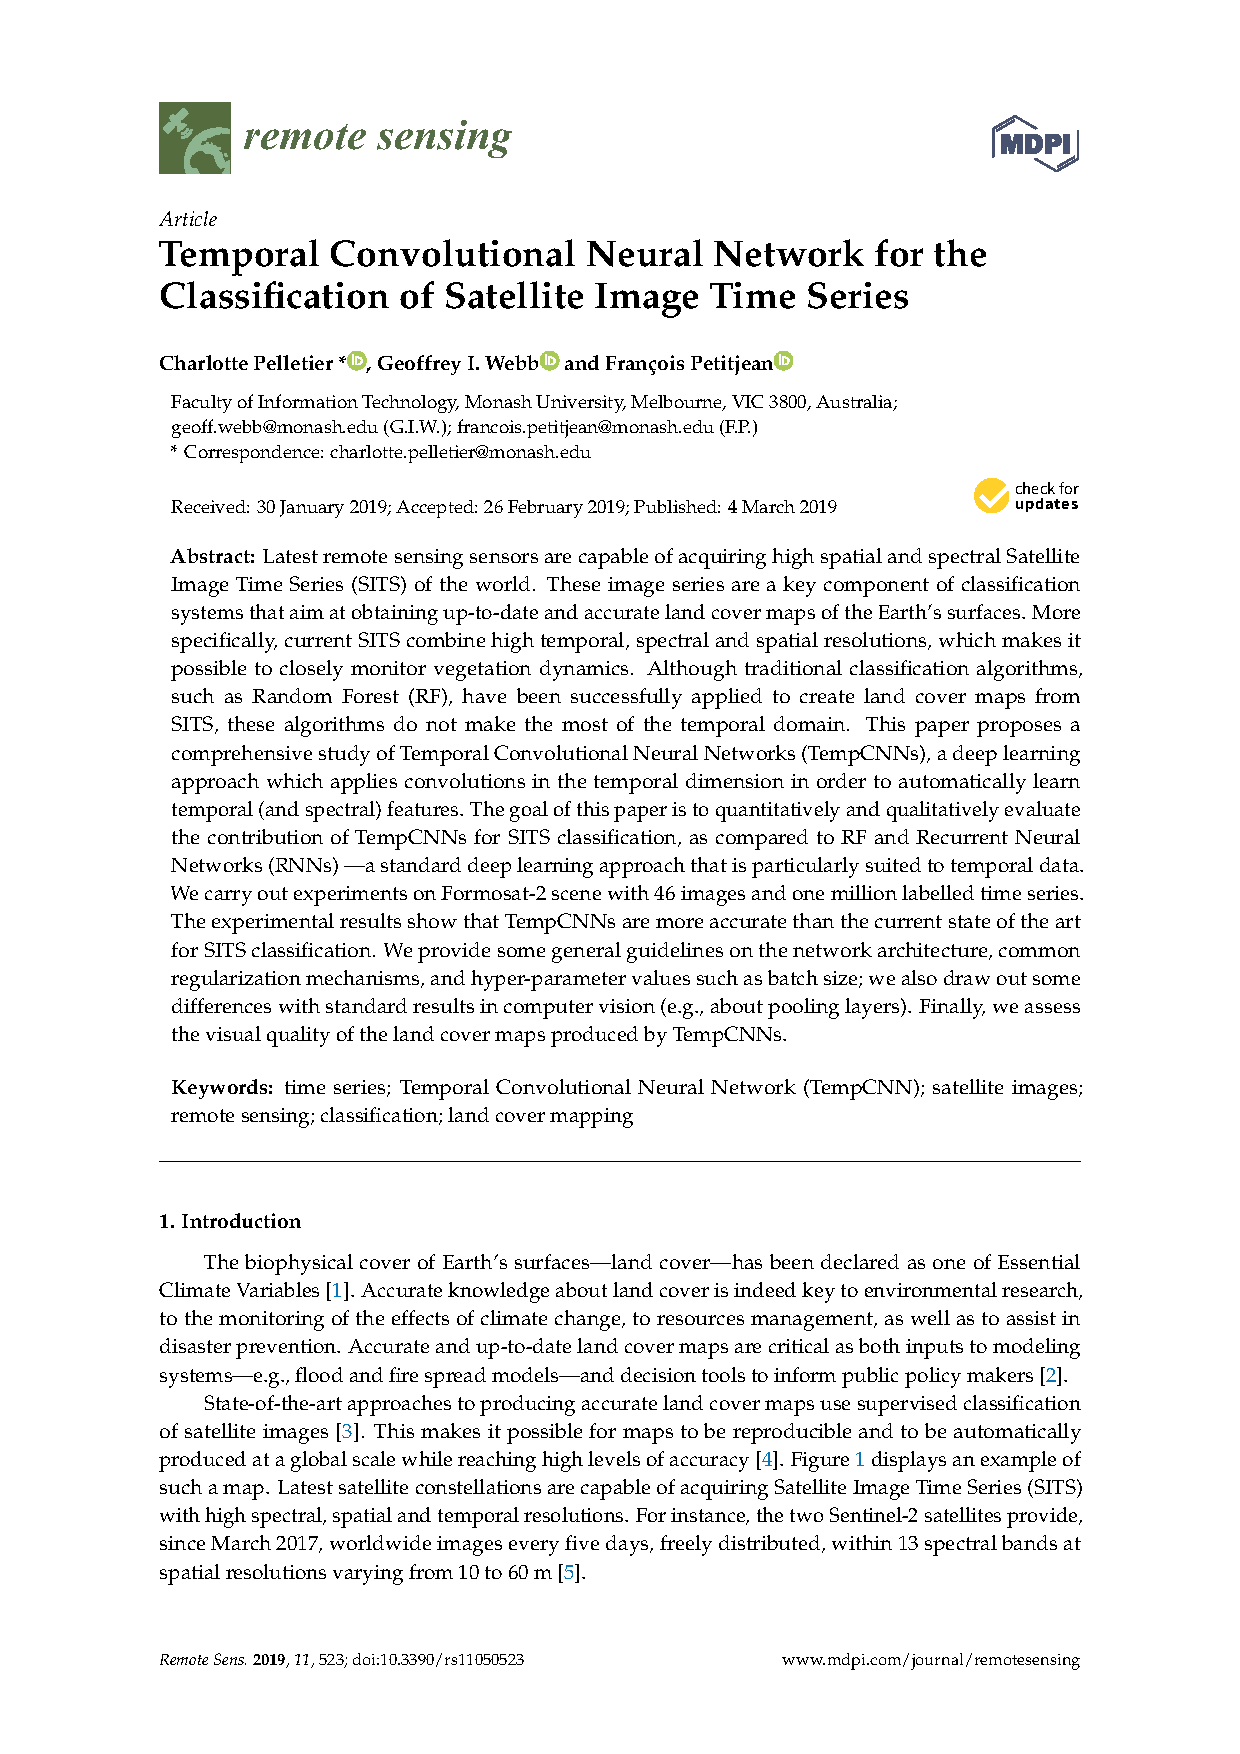
\includegraphics[width=1\textwidth]{tempCNN}
  \caption{Proposed temporal Convolutional Neural Network (TempCNN). The network input is a
  multi-variate time series. Three convolutional filters are consecutively applied, then one dense layer,
  and finally the Softmax layer, that provides the predicting class distribution.    \cite{tempCNN}}
  \label{fig:temCNNArchitecture}
\end{figure}


To prevent overfitting, we employed the same regularization mechanisms described in \cite{tempCNN}:

\begin{itemize}
  \item dropout rate of 0.5 \cite{JMLR:v15:srivastava14a}. 
  \item L2-regularization on the weights (also named weight-decay) applied for all the layers with a small rate of $10^{-6}$ 
  \item batch normalization \cite{DBLP:journals/corr/IoffeS15}.
\end{itemize}

To train the network Adam optimization was used with the standard parameter values: $\beta_1 = 0.9$, $\beta_2 = 0.999$, and $e = 10^{-8}$) \cite{kingma2014adam} 
We used a batch size of 32, and a maximum number of epochs set to 20, with an early stopping mechanism with a patience of zero on the validation loss. 


\subsection{Data preparation}
\label{sec:tempCNNDataPreparation}

The dataset was divided into three subsets: training (60\%), validation (20\%), and test (20\%).
To prevent spatial autocorrelation, we ensured that pixels from the same polygon did not appear in different sets.
We also maintained the similarity of class distribution in each set by keeping the same proportions of classes in the training, validation, and test sets.

% TODO: z-normalization?
To normalize the data, we used min-max normalization, the same used in \cite{tempCNN}.
The traditional min-max normalization performs a subtraction of the minimum, then a division by the range, i.e., the maximum minus the minimum \cite{han2011data}.
This normalization is highly sensitive to extreme values, we propose to use 2\% (or 98\%) percentile rather than the minimum (or the maximum) value. 
For each feature, both percentile values are extracted from all the time-stamp values.

\subsection{Experimental results}

In this section, we present the outcomes of our experiments examining the efficacy of the TempCNN model on time series data from satellite images.
We examined the impact of network depth and the width of its convolutional layers on the classification accuracy. 
Furthermore, we investigated the impact of incorporating pooling layers and filter size on the classification accuracy. 
Finally, we explored the impact of batch size on classification accuracy. 

By thoroughly investigating these factors, we gained insight into how to optimize the TempCNN model for this type of data.


\begin{paragraph}{Depth}
In a convolutional neural network (CNN), the depth refers to the number of layers in the network.
A deeper network can learn more complex features by using a hierarchy of layers, each building on the features learned by the previous layer.
However, increasing the depth can also lead to the vanishing gradient problem, where the gradients become too small to effectively update the weights during training.
Therefore, finding the optimal depth is a crucial consideration when designing a CNN.
\end{paragraph}

To investigate the impact of network depth on model performance while maintaining constant complexity, we vary the number of layers in the network while reducing the number of units in deeper layers.
We experiment with six architectures that consist of between one and six convolutional layers, each with a varying number of units ranging from 256 to 16.
Additionally, each architecture includes one dense layer with a number of units ranging from 64 to 2048. 
In each experiment, we train the model twice: first using the dataset with pre-imputed missing values, and then using a modified dataset where any missing values are replaced with zeros.
As shown in Table \ref{tab:temCNNdepth}, the highest accuracy is achieved with two or three convolutional layers.

\begin{table}[H]
  \centering
   \begin{tabular}{rclrr}
   Model&&                  & No imputation         & Pre imputation             \\[0.2cm]
   \hline \\[-0.2cm]
   1CONV256 &+& 1FC64   	 & $91.39 \pm 0.74$ 	 & $91.12 \pm 0.57$\\
   2CONV128 &+& 1FC128  	 & $91.32 \pm 1.11$ 	 & $91.32 \pm 1.28$\\
   3CONV64 &+& 1FC256   	 & $\mathbf{92.57 \pm 0.84}$ 	 & $\mathbf{92.93 \pm 1.50}$\\
   4CONV32 &+& 1FC512   	 & $92.33 \pm 1.32$ 	 & $90.45 \pm 1.98$\\
   5CONV16 &+& 1FC1024  	 & $91.20 \pm 0.94$ 	 & $88.20 \pm 2.95$\\
   6CONV8 &+& 1FC2048   	 & $87.83 \pm 2.89$ 	 & $88.58 \pm 2.90$\\
   \end{tabular}
   \caption{Influence of depth on classification accuracy.}
   \label{tab:temCNNdepth}
 \end{table}

\begin{paragraph}{Width}
The width of a convolutional neural network (CNN) refers to the number of neurons in each layer.
Increasing the width can enhance the network's ability to learn complex features because more neurons are available for training.
However, a network that is too wide may be prone to overfitting, where it memorizes the training data rather than generalizing to new data.
Therefore, finding the optimal width is critical for achieving the best performance on the test data.
\end{paragraph}

To evaluate the impact of width on model performance, we experimented with seven CNN architectures.
Each architecture includes three convolutional layers, one dense layer with 256 neurons, and a Softmax layer, as illustrated in Figure \ref{fig:temCNNArchitecture}.
The architectures differ in the number of parameters, and we vary the width of the convolutional layers from 16 to 1024 neurons.

 \begin{table}[H]
  \centering
   \begin{tabular}{rclrr}
   Model&&                  & No imputation         & Pre imputation             \\[0.2cm]
   \hline \\[-0.2cm]
   3CONV16 &+& 1FC256    	 & $92.44 \pm 0.83$ 	 & $91.62 \pm 0.41$\\
   3CONV32 &+& 1FC256    	 & $92.52 \pm 0.68$ 	 & $92.16 \pm 0.68$\\
   3CONV64 &+& 1FC256    	 & $92.45 \pm 0.89$ 	 & $\mathbf{93.47 \pm 0.63}$\\
   3CONV128 &+& 1FC256   	 & $92.26 \pm 1.84$ 	 & $92.13 \pm 1.35$\\
   3CONV256 &+& 1FC256   	 & $91.66 \pm 1.96$ 	 & $92.04 \pm 1.67$\\
   3CONV512 &+& 1FC256   	 & $91.97 \pm 1.23$ 	 & $92.75 \pm 1.73$\\
   3CONV1024 &+& 1FC256  	 & $\mathbf{92.76 \pm 1.46}$ 	 & $93.39 \pm 1.54$\\
   \end{tabular}
   \caption{Influence of width on classification accuracy.}
   \label{tab:temCNNwidth}
 \end{table}

The results reported in Table \ref{tab:temCNNwidth} show that the architecture is remarkably robust, even when there is considerable variation in the number of neurons.
This is illustrated by the fact that the overall accuracy shows a difference of only 1.7\% between the model with lower parameters and the one with higher parameters when using pre-imputed data, while the difference is only 0.32\% when there is no imputation for missing values.
Although the standard deviation increases with the number of parameters, the architecture consistently achieves high accuracy rates, indicating that it is capable of maintaining good performance even with a larger number of neurons.

We opted to utilize the model with three convolutional layers, each with 64 neurons, and one dense layer comprising 256 neurons for the upcoming experiments because it offers a favorable balance between bias and variance.
This choice was made with consideration to the size of our training dataset, which comprises 80,000 samples.

\begin{paragraph}{Batch size}
In machine learning, batch size refers to the number of training examples used in an iteration of gradient descent.
The batch size plays a crucial role in determining the efficiency and accuracy of the training process.
A larger batch size can result in faster training because the algorithm can process more examples in each iteration.
However, using a larger batch size can also lead to a less accurate model because it can cause the optimization algorithm to converge to a suboptimal solution.
On the other hand, using a smaller batch size may result in slower training, but may help the algorithm converge to a better solution. 
Thus, choosing an appropriate batch size is an important consideration in machine learning.
\end{paragraph}

We conducted experiments to determine the optimal batch size for training the TempCNN model.
Specifically, we tested four different batch sizes: 16, 32, 64, and 128.
Our analysis, as presented in Table \ref{tab:temCNNbatchsize}, shows that batch size has a noticeable impact on training time; larger batch sizes result in faster training times.
However, we observed that the batch size does not have a significant effect on the overall accuracy of the TempCNN model.
In fact, we found that the accuracy values for all four batch sizes are comparable, indicating that selecting an appropriate batch size is not a critical factor in achieving high accuracy for this model.

\begin{table}[H]
  \centering
   \begin{tabular}{rlll}
   Batch size                 & Train time  & No imputation         & Pre imputation             \\[0.2cm]
   \hline \\[-0.2cm]
    16        & 52min  	 & $91.92 \pm 1.50$ 	 & $92.16 \pm 1.75$\\
    32        & 42min  	 & $\mathbf{91.61 \pm 1.19}$ 	 & $\mathbf{93.74 \pm 0.03}$\\
    64        & 26min  	 & $90.88 \pm 1.63$ 	 & $92.30 \pm 0.89$\\
    128       & 20min  	 & $91.54 \pm 1.69$ 	 & $91.52 \pm 1.67$\\
   \end{tabular}
   \caption{Influence of batch size on training time and classification accuracy.}
   \label{tab:temCNNbatchsize}
 \end{table}
 
\begin{paragraph}{Pooling layers}
Pooling is a common technique used in deep learning for dimensionality reduction and feature extraction.
In the context of computer vision, the two most popular types of pooling are local max-pooling \cite{Ren2015Faster} and global average pooling \cite{He2016Deep}.
Local max-pooling takes the maximum value of a small subregion of a feature map, while global average pooling takes the average of all feature map values.
However, for time series data, global average pooling has been shown to be more effective in previous studies \cite{rs10020236,fawaz2018deep}.
In this work, we investigate whether these findings can be generalized to time series classification tasks. 
Specifically, we will compare the performance of the TempCNN model using both local max-pooling and global average pooling to determine which pooling method is most effective for our specific application.
\end{paragraph}

\begin{paragraph}{Filter size}
Filter Size is an important Hyperparameter in Convolutional Neural Networks (CNNs)
The filter size, also known as the kernel size, determines the receptive field of the convolutional layer and influences the network's ability to capture spatial features in the input.
A larger filter size allows the network to capture more complex patterns and details, but at the cost of increased computation and potential overfitting.
Conversely, a smaller filter size reduces computation and may improve the network's ability to generalize to new data, but at the risk of losing important features.
Therefore, the filter size should be chosen based on the complexity of the task and the size of the input data.
\end{paragraph}



Figure \ref{tab:tempCNNPooling} displays the OA values as a function of filter size. 
Each bar represents a different configuration: local max-pooling (MP), local max-pooling and global average pooling (MP + GAP), local average pooling (AP), local and global average pooling (AP + GAP), and global average pooling (GAP). 
The horizontal magenta dashed line corresponds to the OA values obtained without pooling layers in the previous experiment.


\begin{figure}[H]
  \centering
  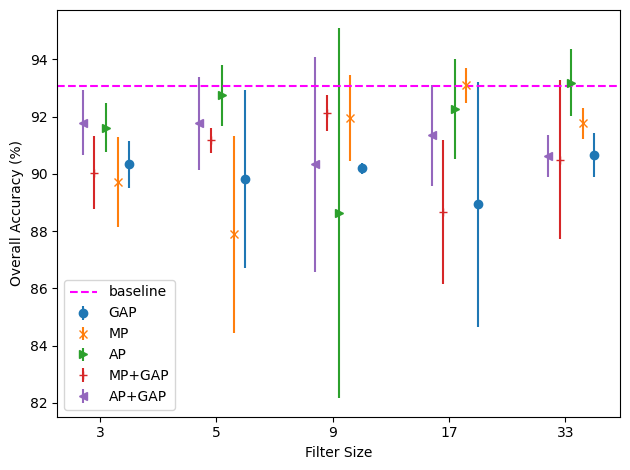
\includegraphics[width=0.7\textwidth]{tempCNNPooling.png}
  \caption{Overall Accuracy as a Function of Filter Size for Different Pooling Methods: Local max-pooling (MP) in orange, local max-pooling and global average pooling (MP + GAP) in red, local average pooling (AP) in green, local and global average pooling (AP + GAP) in purple, and global average pooling (GAP) in blue.}
  \label{tab:tempCNNPooling}
\end{figure}

Figure \ref{tab:tempCNNPooling} shows that the use of pooling layers performs poorly: the OA results are almost always
below the one obtained without pooling layers (magenta dashed line). 

\subsection{Findings}

Our experiments on the TempCNN model for satellite image time series data have provided some valuable insights. 
First, we found that a network depth of 3 layers is sufficient to achieve high classification accuracy. 
Additionally, we discovered that a width of 64 neurons per layer is adequate. 
Furthermore, we determined that a batch size of 32 is sufficient for training the model. 
Finally, we observed that the use of pooling layers did not contribute significantly to the classification accuracy.

The model has been implemented in Python using the Keras library \cite{chollet2015keras} and the TensorFlow backend \cite{tensorflow2015-whitepaper}.
The source code for this model is accessible at \url{https://github.com/dnldsht/temporalCNN}, which is a forked version of the initial TempCNN implementation \cite{tempCNN}.